\documentclass[a4paper, 10pt]{report}
\usepackage[italian]{babel}
\usepackage[T1]{fontenc}
\usepackage[utf8]{inputenc}
\usepackage{charter}
\usepackage{amsmath}
\usepackage{amsthm}
\usepackage{amsfonts}
\usepackage{graphicx}
\usepackage{wrapfig}
\usepackage{tcolorbox}
\usepackage{fancyhdr}
\usepackage{longtable}

\usepackage{geometry}
\geometry{a4paper, left=2cm,right=2cm,top=2cm,bottom=2cm}

\pagestyle{fancy}
\lhead{}
\chead{}
\rhead{\bfseries 08 ottobre 2019}
\lhead{\bfseries Basi di dati}


\begin{document}

\section*{\underline{Modello Entità - Relazione}}

Il modello Entità - Relazione è un modello per la progettazione di basi di dati. I suoi costrutti del sono i seguenti:\\

\begin{longtable}{| p{.10\textwidth} | p{.80\textwidth} |} 
\textbf{Entità} & Rappresenta una classe di oggetti (simile a quella dei linguaggi ad oggetti) che presenta tre caratteristiche principali: ha esistenza autonoma, ha proprietà comuni, ha identificazione univoca.

A livello grafico, un'entità $E$ viene rappresentata come un RETTANGOLO con all'interno il nome dell'entità stessa:

\begin{center}
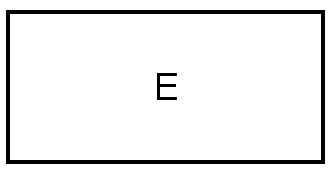
\includegraphics[scale=0.4]{img1.pdf}
\end{center}

Un'istanza (o occorrenza) di un'entità $E$ è ogni oggetto che appartiene alla classe rappresentata da $E$. L'insieme delle istanze di $E$ si indica con $I(E)$.

\underline{Esempio}:

\begin{center}
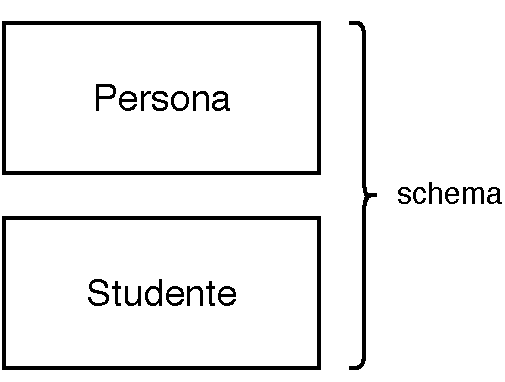
\includegraphics[scale=0.4]{img2.pdf}
\hspace{1cm}
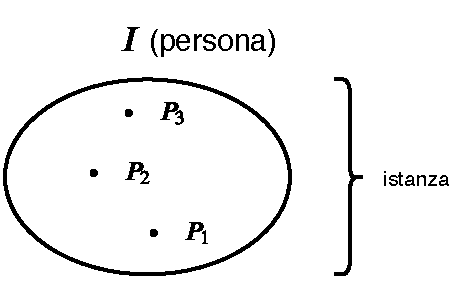
\includegraphics[scale=0.5]{img3.pdf}
\end{center}

Osservazioni:
\begin{enumerate}
\item Inizialmente l'insieme delle istanze di un'entità $E$ è vuoto -> $I(E) = \emptyset$;
\item Ogni istanza di $E$ nasce e muore nella base di dati in modo indipendente dalle altre entità;
\item Ogni oggetto che rappresenta un'istanza di entità ha un'esistenza autonoma rispetto alle sue proprietà -> il modello ER è orientato agli oggetti.
\end{enumerate}\\

\textbf{Relazione} & Rappresenta un legame logico tra 2 o più proprietà.

La rappresentazione grafica di una relazione $R$ tra le entità $E_1,..., E_n$ si ha tramite un ROMBO collegato attraverso una spezzata a ciascuna delle entità. Il nome della relazione viene indicato vicino al rombo.

\begin{center}
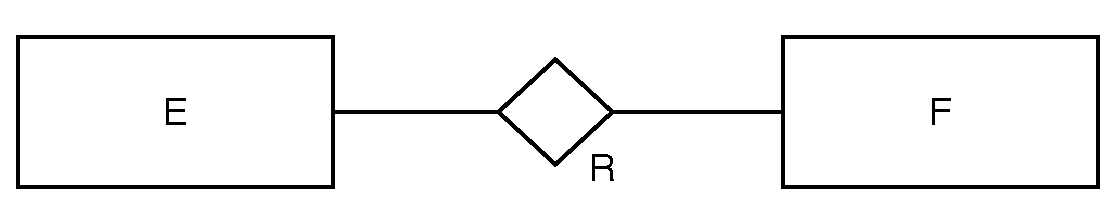
\includegraphics[scale=0.35]{img4.pdf}

(Relazione binaria)

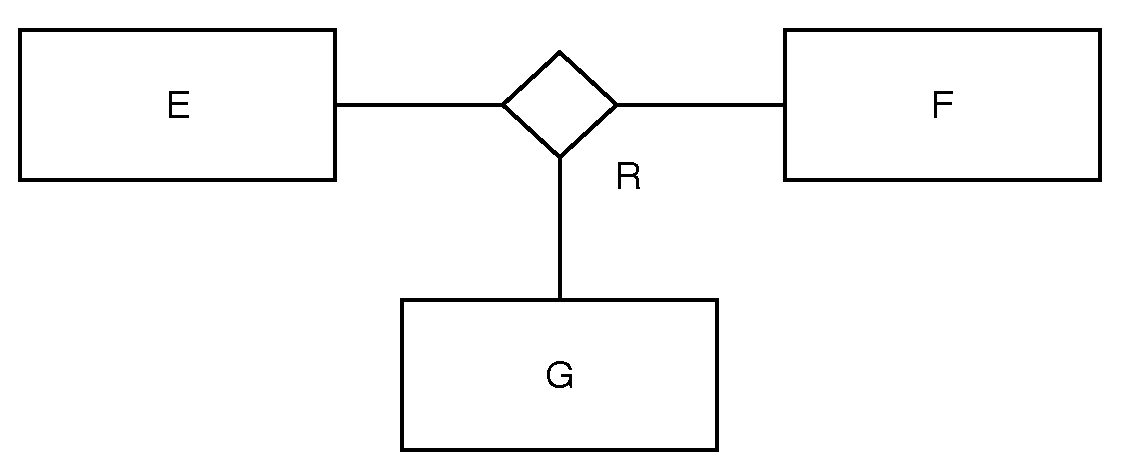
\includegraphics[scale=0.35]{immagine5.pdf}

(Relazione ternaria)

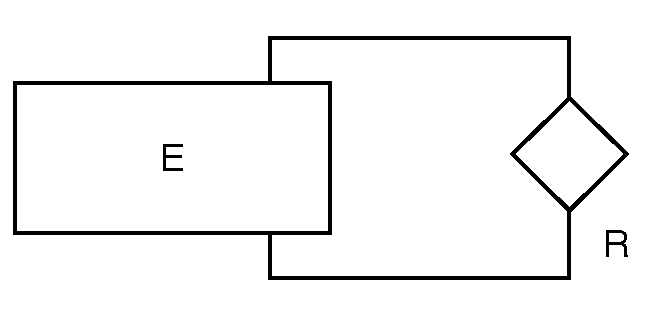
\includegraphics[scale=0.35]{immagine6.pdf}

(Relazione ricorsiva)
\end{center}

Un'istanza di una relazione $R$ è la ennupla di occorrenze delle entità $E_1,..., E_n$ definita come: $r = (e_1,..., e_n)$ con $e_i \in I(E_i)$ per $1 \le i \le n$.
\end{longtable}

\begin{longtable}{| p{.10\textwidth} | p{.80\textwidth} |} 
 & \underline{Esempio}:

\begin{center}
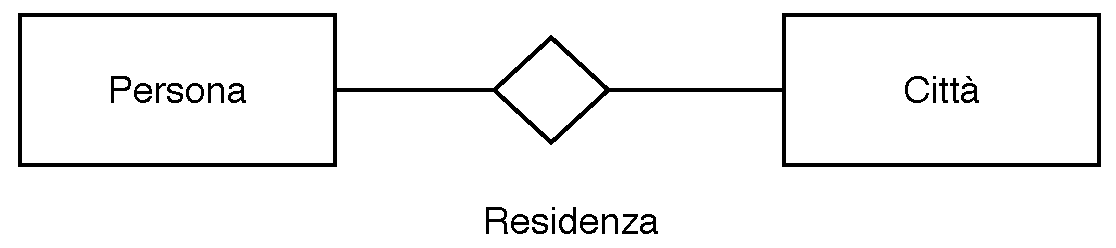
\includegraphics[scale=0.40]{immagine7.pdf}

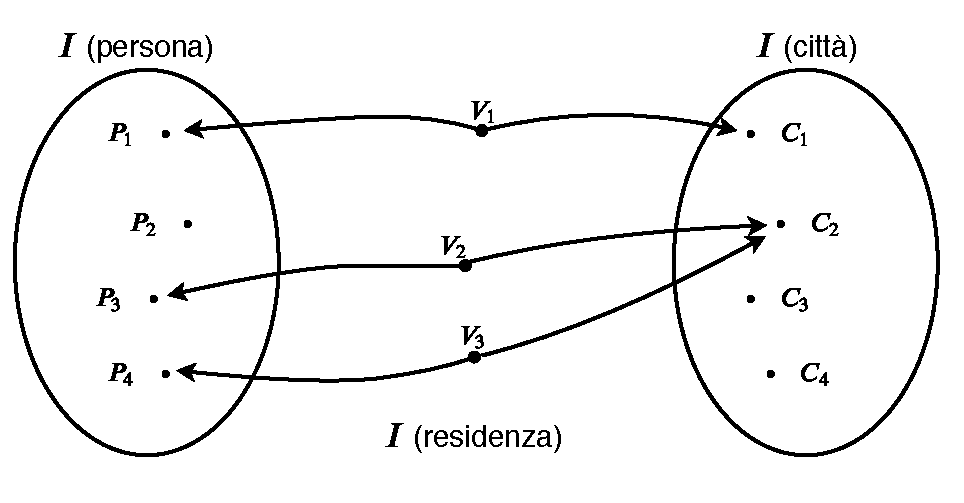
\includegraphics[scale=0.40]{immagine8.pdf}
\end{center}

Osservazioni:
\begin{enumerate}
\item Inizialmente l'insieme delle istanre di una relazione $R$ è vuoto -> $I(R) = \emptyset$;
\item Per istanziare una relazione $R$ che coinvolge le entità $E_1,..., E_n$ è necessario che esista almeno un'istanza delle entità $E_1,..., E_n$;
\item Data una relazione $R$ sulle entità $E_1,..., E_n$, allora $I(R) \subseteq I(E_1) x ... x I(E_n)$.
\end{enumerate}\\

\textbf{Attributo} & Rappresenta una prorpietà elementare delle istanze o delle relazioni. Ogni attributo $a$ associa uno ed un solo valore ad ogni istanze di $E$ o $R$ appartenente ad un dominio (ovvero all'insieme dei valori ammissibili). Si può quindi rappresentare come una funzione: $f_a : I(E) \rightarrow DOMINIO$.

Un attributo si rappresenta, graficamente, tramite un PALLINO VUOTO collegato all'entità o alla relazione tramite una spezzata:

\begin{center}
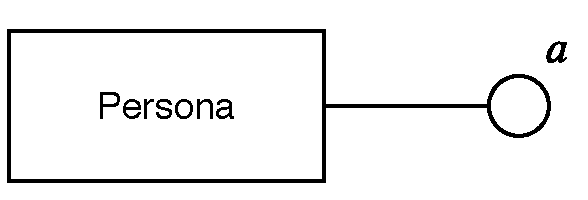
\includegraphics[scale=0.40]{immagine9.pdf}

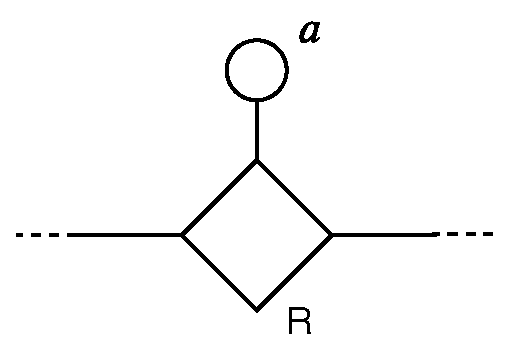
\includegraphics[scale=0.40]{immagine10.pdf}
\end{center}

ATTENZIONE: di norma un attributo non può essere nullo.

\underline{Esempio}:

\begin{center}
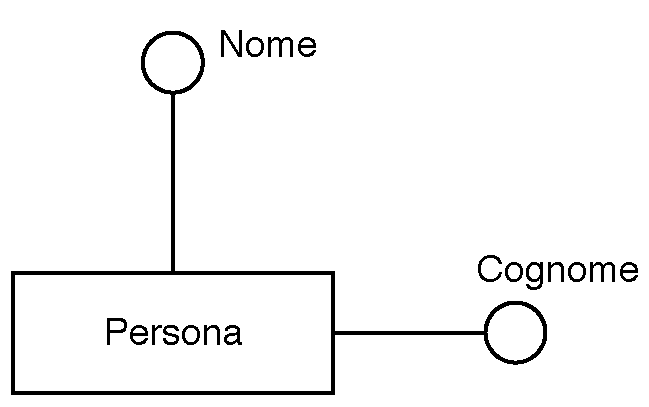
\includegraphics[scale=0.40]{immagine11.pdf}
\end{center}

\end{longtable}


\end{document}
